\section{Towards Quantum Field Theory}

The concept of a \textbf{field} is central to modern physics, describing how physical quantities vary over space and time. It was introduced in the 19th century to explain phenomena such as electromagnetism and gravity, in order to move away from the idea of \textit{action at a distance}:
\begin{itemize}
  \item The \textbf{gravitational field}, described by Newton's law of universal gravitation, which explains the attraction between masses.
  \item The \textbf{electromagnetic field}, unified by Maxwell's equations, which describes electric and magnetic phenomena and their interactions with charged particles.
\end{itemize}
In this framework, particles interact locally through fields, rather than instantaneously over a distance.

Photons, the quanta of the electromagnetic field, mediate electromagnetic interactions; they represent the field's excitations around its ground state, thus allowing for the exchange of energy and momentum between charged particles. This description seems to elect the field as the fundamental entity, with particles being secondary manifestations. However, matter particles, such as electrons and quarks, seem to be more fundamental, as they constitute the building blocks of matter. This duality raises the question: which is more fundamental, fields or particles?\footnote{If we were to choose particles as fundamental, we would face the challenge of explaining how they interact at a distance, and fields like the EM one would be described as classical limits of a collection of photons.}

Quantum Field Theory provides a framework in which \textbf{fields are the fundamental quantities} and particles are viewed as excitations of underlying fields that permeate space and time, rather than as independent entities. Each type of particle corresponds to a specific field:
\begin{itemize}
    \item The \textbf{EM field} gives rise to photons, which mediate electromagnetic interactions.
    \item The \textbf{electron field} (Dirac) gives rise to electrons and positrons.
    \item The \textbf{quark fields} (Dirac) give rise to quarks, which combine to form protons and neutrons.
    \item The \textbf{Higgs field} (Klein-Gordon) is responsible for giving mass to particles through the Higgs mechanism.
\end{itemize}
Particles are thus seen as localized excitations or quanta of their respective fields around their ground states, and interactions between particles are understood as interactions between these fields.

\subsection*{Properties of the New Approach}

The new framework of QFT has several important properties, which are granted by the formulation itself:
\begin{enumerate}[label=(\roman*),align=left,itemsep=1.0\baselineskip]
    \item \textbf{Locality}:\\
    Interactions occur at specific points in space and time, ensuring that cause and effect are preserved.
    
    \item \textbf{Causality}:\\
    No information or influence can travel faster than the speed of light, preserving the causal structure of spacetime. 
    \item \textbf{Particle/antiparticle creation/annihilation}:\\
    
    \item \textbf{Undistinguishability of particles of identical type}:\\
    
    \item \textbf{Correct spin-statistics relations}:\\
\end{enumerate}

\subsection*{Units and Scales}

\dots

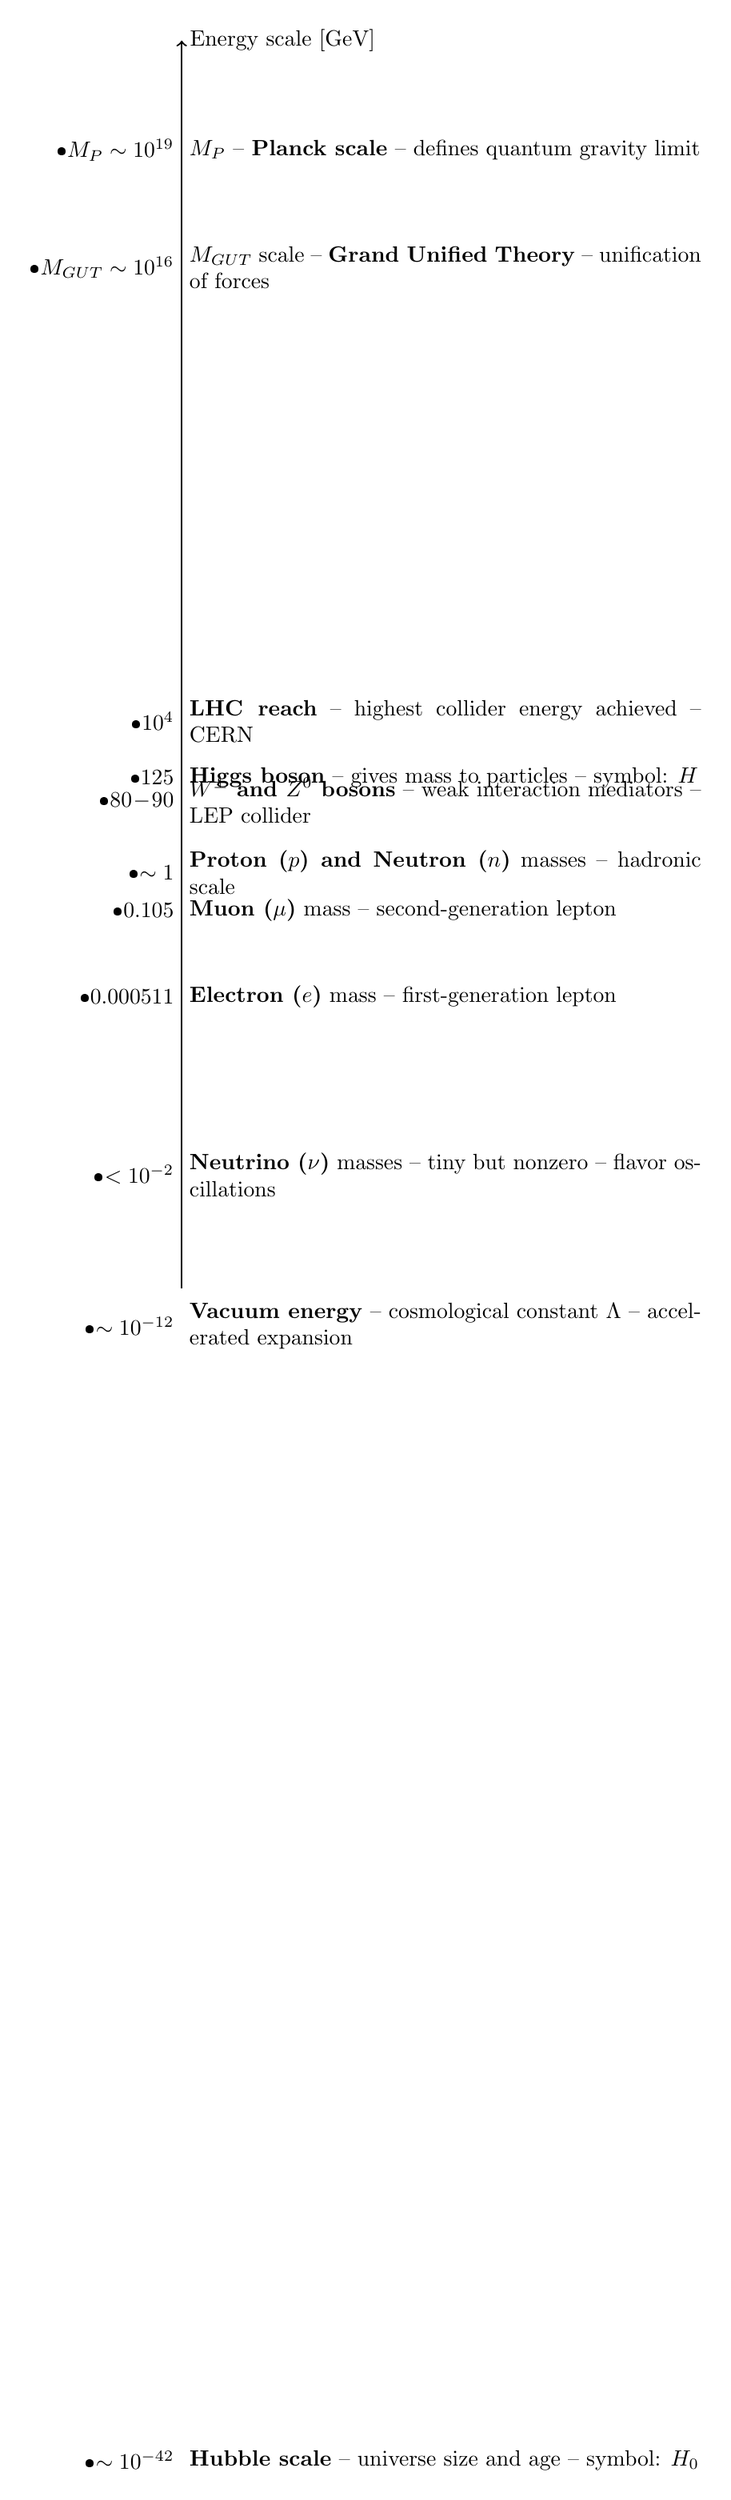
\begin{tikzpicture}[x=0cm,y=0.6cm]

  \draw[thick,->] (-1,7) -- (0,40) node[anchor=west]{Energy scale [GeV]};

  \foreach \y/\E/\desc in {
    18.1/{$M_P \sim 10^{19}$}/ $M_P$ -- \textbf{Planck scale} -- defines quantum gravity limit,
    15/{$M_{\text{GUT}} \sim 10^{16}$}/$M_{\text{GUT}}$ scale -- \textbf{Grand Unified Theory} -- unification of forces,
    3/{$10^4$}/\textbf{LHC reach} -- highest collider energy achieved -- CERN,
    1.5/{$125$}/\textbf{Higgs boson} -- gives mass to particles -- symbol: $H$,
    0.9/{$80\!-\!90$}/\textbf{$W^\pm$ and $Z^0$ bosons} -- weak interaction mediators -- LEP collider,
    -1/{$\sim 1$}/\textbf{Proton ($p$) and Neutron ($n$)} masses -- hadronic scale,
    -2/{$0.105$}/\textbf{Muon ($\mu$)} mass -- second-generation lepton,
    -4.3/{$0.000511$}/\textbf{Electron ($e$)} mass -- first-generation lepton,
    -9/{$<10^{-2}$}/\textbf{Neutrino ($\nu$)} masses -- tiny but nonzero -- flavor oscillations,
    -13/{$\sim 10^{-12}$}/\textbf{Vacuum energy} -- cosmological constant $\Lambda$ -- accelerated expansion,
    -43/{$\sim 10^{-42}$}/\textbf{Hubble scale} -- universe size and age -- symbol: $H_0$
  }{
    \pgfmathsetmacro{\yy}{\y + 19}
    \draw (-1.15,\yy) -- (0.15,\yy);
    \node[anchor=east] at (-1.2,\yy) {\textbullet \E};
    \node[anchor=west,text width=\textwidth-4cm,align=justify] at (0.3,\yy) {\desc};
  }

\end{tikzpicture}



\section{Mechanical Model of a Quantum Field}